%\documentclass[ps,gyom,slideColor,colorBG,total]{prosper}
\documentclass[pdf,gyom,slideColor,colorBG,total]{prosper}
%\documentclass[pdf,gyom,slideColor,colorBG,total,accumulate]{prosper}
\usepackage{amsmath}
\usepackage{textcomp}
\usepackage{mathptmx}
\usepackage[scaled]{helvet}
\usepackage{courier}
\title{A Principle Compiler for Extensible Dependency Grammar}
\subtitle{Bachelor Thesis\\ {Programming Systems Lab}}
\author{\texttt{Jochen Setz, 24.05.2007 \\ Betreuer: Ralph Debusmann}}
\date{24.05.2007}
\slideCaption{A Principle Compiler for Extensible Dependency Grammar}
%\institution{Universit{\"a}t Hamburg}
%\DefaultTransition{Dissolve}
\bibliographystyle{alpha}
\begin{document}
\maketitle
\overlays{5}{
\begin{slide}{Extensible Dependency Grammar}
\begin{itemstep}
\item Grammatikformalismus f\"ur Dependenzgrammatik
\item Modell: Tupel von Dependenzgraphen
\item Dependenzgraphen hei{\ss}en Dimensionen
\item alle Dimensionen haben die gleiche Knotenmenge
\end{itemstep}
\fromSlide{5}{
$\Rightarrow$ Modelle = Multigraphen
}
\end{slide}
}


\overlays{1}{
\begin{slide}{XDG Beispiel}
{\begin{figure}[!ht]
\centering
\begin{tabular}{cc}
  \small{\textsc{SYN:}} & \\
 &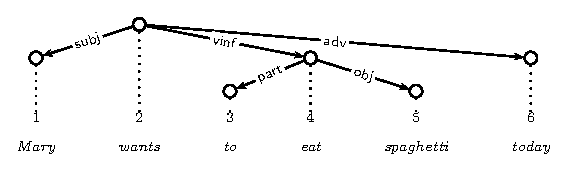
\includegraphics[width=7cm]{xdg_syn.eps}\\
      \small{\textsc{SEM:}} & \\
 & 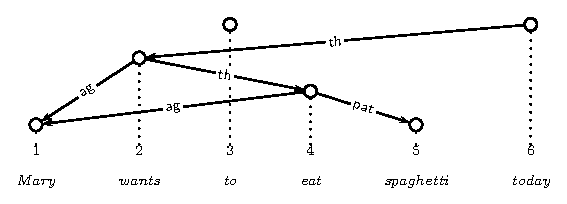
\includegraphics[width=7cm]{xdg_sem.eps}\\
    \end{tabular}%
%    \caption{Beispiel}\label{xdg}%
\end{figure}}

\end{slide}
}


\overlays{4}{
\begin{slide}{Prinzipien}
\begin{itemstep}
\item Wohlgeformtheitbedingungen f\"ur Multigraphen
\end{itemstep}
\fromSlide{2}{
Beispiele:}
\begin{itemize}
\fromSlide{2}{
\item Baumheit (eine Wurzel / keine Zyklen / \\
keine oder eine Mutter pro Knoten)}
\fromSlide{3}{
\item Valenz (Anzahl und Art der ein-/ausgehenden Kanten)}
\fromSlide{4}{
\item Projektivit\"at (keine kreuzenden Kanten)}
\end{itemize}
\end{slide}
}



\overlays{2}{
\begin{slide}{Prinzipien in FOL}
\begin{itemstep}
\item Prinzipien in First Order Logic (FOL) formalisiert
\end{itemstep}
\fromSlide{2}{
Z.B. Baumheit auf Dimension $d$:

\begin{itemize}
\item $NoCycles = \forall v : \neg (v \rightarrow ^+ _d v)$
\item $OneRoot = \exists^1 v : \neg \exists v' : v' \rightarrow _d v$
\item $ZeroOrOneMother =$ \\
$ \forall v : (\neg \exists v' : v' \rightarrow _d v) \vee (\exists^1 v' : v' \rightarrow _d v)$
\end{itemize}
}
\end{slide}
}
\begin{slide}{XDK}
\centering

\includegraphics[width=8.5cm]{xdk.eps}
\end{slide}

{\overlays{3}{
\begin{slide}{Parser (Grundidee)}
\begin{itemize}
\fromSlide{1}{
\item Multigraphen kodiert durch endliche Mengen von Integern}
\fromSlide{2}{
\item jeder Knoten v mit einem Index und verschiedenen Mengen assoziiert, z.B.:
{\small
\begin{itemize}
\item mothers: Mutterknoten von v
\item daughters: T\"ochter von v
\item up: Vorfahren von v
\item daughtersL: Menge von Tupeln, jedes Tupel hat das gleiche Label
\end{itemize}}
}
\fromSlide{3}{
\item Prinzipien: Constraints auf diesen Mengen}
\end{itemize}
\end{slide}
}

{\overlays{4}{
\begin{slide}{Implementierung von Prinzipien}
\begin{itemstep}
\item Prinzipien m\"ussen von Hand als Mozart/Oz-Constraints implementiert werden
\item $\Rightarrow$ nur Experten in Mozart/Oz und XDK k\"onnen neue Prinzipien schreiben, nicht aber typische Anwender wie z.B. Linguisten
\item $\Rightarrow$ gro{\ss}e L\"ucke zwischen Formalisierung und
  Implementierung
\item provisorische Br\"ucke: umfangreiche Bibliothek von vorimplementierten Prinzipien
\end{itemstep}
\end{slide}
}


\overlays{4}{
\begin{slide}{Idee meiner BA-Thesis}
\begin{itemstep}
\item L\"ucke zwischen Formalisierung und Implementierung schlie{\ss}en
\item Ziel: Compiler (``PrincipleWriter''), der in FOL geschriebene
  Prinzipien in Mozart/Oz- Constraints \"ubersetzt, und ins XDK
  integriert
\item dadurch XDK attraktiver f\"ur typische Anwender, die neue
  Prinzipien schreiben wollen: nur noch Kenntnisse in FOL ben\"otigt
\item Nebeneffekt: Formalisierung und Implementierung r\"ucken n\"aher zusammen
\end{itemstep}
\end{slide}
}


\overlays{4}{
\begin{slide}{Arbeitspakete}
\begin{itemize}
\fromSlide{1}{
\item konkrete Eingabesyntax definieren (fertig)}
\fromSlide{2}{
\item Mozart/Oz-Constraints f\"ur FOL finden (1.~Version)}
\fromSlide{3}{
\item Compiler bauen, der Eingabesyntax in Mozart/Oz-Constraints \"uberf\"uhrt, mit
\begin{itemize}
\item Typ-Checker,
\item Typ-Inferenz
\end{itemize}
}
\end{itemize}
\fromSlide{4}{
{\Large {\color{red}Wie gut kann der PrincipleWriter optimieren, verglichen mit einem Experten?}}
}

\end{slide}
}

\begin{slide}{Literatur}
\begin{itemize}
\item Ralph Debusmann (2006). Extensible Dependency Grammar: A Modular Grammar Formalism Based On Multigraph Description. PhD thesis (revised version)
\item Ralph Debusmann (2007). Scrambling as the Intersection of Relaxed Context-Free Grammars in a Model-Theoretic Grammar Formalism. ESSLLI 2007 Workshop Model Theoretic Syntax at 10, Dublin
\end{itemize}
\end{slide}

\begin{slide}{Optimierung - ZeroOrOneMother}

FOL:
\[ \forall v : (\neg \exists v' : v' \rightarrow _d v) \vee (\exists^1 v' : v' \rightarrow _d v)
\]
UL: 
\begin{verbatim}
forall V::node:
  ~exists V1::node: edge(V1 V D)
  | 
  existsone V1::node: edge(V1 V D)
\end{verbatim}
\end{slide}

\begin{slide}{Optimierung - ZeroOrOneMother}
Mozart/Oz: 
\[
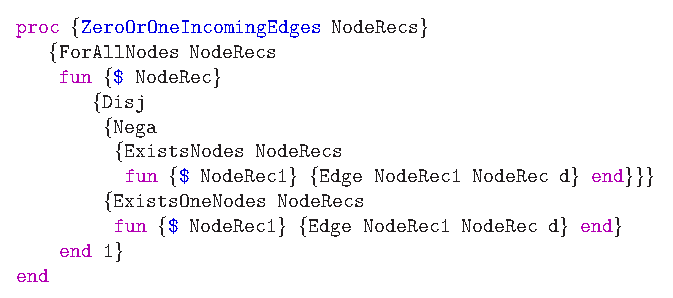
\includegraphics[width=10cm]{zeroorone.eps}
\]
Komplexit\"at: O(n$^2$)
\end{slide}

\begin{slide}{Optimierung - ZeroOrOneMother}
FOL: $ \forall v : \underbrace{(\neg \exists v' : v' \rightarrow _d v)}_{|mothers(v)|~=~0} \vee \underbrace{(\exists^1 v' : v' \rightarrow _d v)}_{|mothers(v)|~=~1}$\\[1cm]
Optimiert: $\forall v: ~ |mothers(v)| ~ \leq ~ 1$\\[1cm]
Komplexit\"at: O(n)
\end{slide}

\end{document}

